\documentclass[11pt]{article}

\usepackage[margin=1in]{geometry}
\usepackage{amsmath,amssymb,amsfonts}
\usepackage{graphicx}
\usepackage{booktabs}
\usepackage{float}
\usepackage{siunitx}
\usepackage{array}
\usepackage{hyperref}
\usepackage{enumitem}
\usepackage{caption}
\usepackage{xcolor}

\hypersetup{
    colorlinks=true,
    linkcolor=blue,
    citecolor=blue,
    urlcolor=blue
}

\title{\textbf{SES 598 --- Assignment 2\\
Cart-Pole Optimal Control Under Earthquake Disturbance}}
\author{Aaryan Anand}
\date{\today}

\begin{document}

\maketitle

\begin{abstract}
This report presents the design and tuning of a Linear Quadratic Regulator (LQR) for an inverted cart-pole system subject to continuous earthquake-like disturbances in simulation. The controller was initialized using Bryson's Rule and then manually refined to improve robustness, reduce oscillation, and improve recovery from difficult initial conditions. The final controller was selected based on consistency across repeated trials rather than the best single run. Performance was evaluated using stable operation duration, maximum cart displacement, maximum pole angle deviation, and control effort.
\end{abstract}

\section{Introduction}
The objective of this assignment was to analyze and tune an LQR controller for a cart-pole system in the presence of external earthquake disturbances. The cart-pole is a standard unstable system in control theory, since the pole must be maintained near the upright equilibrium while the cart remains within finite rail limits.

In this assignment, the controller had to satisfy competing objectives:
\begin{itemize}[itemsep=2pt]
    \item maintain the pendulum near the upright position,
    \item keep the cart within its physical range of motion,
    \item reject continuous disturbance forces,
    \item and avoid excessive control effort.
\end{itemize}

The initial controller was generated using Bryson's Rule to obtain a principled first-pass choice of $Q$ and $R$. The controller was then manually tuned by observing failure modes, transient behavior, oscillation, and consistency across multiple trials.

\section{System Description}
The system consists of an inverted pendulum mounted on a cart constrained to move horizontally. The simulated model parameters are:
\begin{itemize}[itemsep=2pt]
    \item cart mass: $M = \SI{1.0}{kg}$,
    \item pole mass: $m = \SI{1.0}{kg}$,
    \item pole length: $L = \SI{1.0}{m}$,
    \item gravitational acceleration: $g = \SI{9.81}{m/s^2}$,
    \item cart travel range: $\pm \SI{2.5}{m}$.
\end{itemize}

The system is also subject to an external earthquake disturbance modeled as a time-varying force with randomized frequency, amplitude variation, phase shifts, and additive noise.

\section{LQR Background}
The cart-pole was controlled using full-state feedback of the form
\begin{equation}
    u = -Kx
\end{equation}
where $x$ is the state vector and $u$ is the horizontal force applied to the cart.

The state vector was defined as
\begin{equation}
    x = \begin{bmatrix}
        x & \dot{x} & \theta & \dot{\theta}
    \end{bmatrix}^T
\end{equation}
where:
\begin{itemize}[itemsep=2pt]
    \item $x$ is cart position,
    \item $\dot{x}$ is cart velocity,
    \item $\theta$ is pole angle,
    \item $\dot{\theta}$ is pole angular velocity.
\end{itemize}

The linearized state-space model used in the provided controller is
\begin{equation}
    \dot{x} = Ax + Bu
\end{equation}
with
\begin{equation}
A =
\begin{bmatrix}
0 & 1 & 0 & 0\\
0 & 0 & \frac{mg}{M} & 0\\
0 & 0 & 0 & 1\\
0 & 0 & \frac{(M+m)g}{ML} & 0
\end{bmatrix},
\qquad
B =
\begin{bmatrix}
0\\
\frac{1}{M}\\
0\\
-\frac{1}{ML}
\end{bmatrix}.
\end{equation}

The LQR controller minimizes the quadratic cost function
\begin{equation}
    J = \int_0^\infty \left( x^TQx + u^TRu \right) dt
\end{equation}
where $Q$ penalizes state deviations and $R$ penalizes control effort.

\section{Bryson's Rule Initialization}
A first-pass controller was generated using Bryson's Rule, which sets the state and input weights based on maximum acceptable values:
\begin{equation}
Q = \mathrm{diag}\left(
\frac{1}{x_{\max}^2},
\frac{1}{\dot{x}_{\max}^2},
\frac{1}{\theta_{\max}^2},
\frac{1}{\dot{\theta}_{\max}^2}
\right),
\qquad
R = \begin{bmatrix}
\frac{1}{u_{\max}^2}
\end{bmatrix}.
\end{equation}

This approach provides a physically interpretable starting point:
\begin{itemize}[itemsep=2pt]
    \item smaller allowable state values produce larger penalties,
    \item larger allowable input values reduce the penalty on control effort.
\end{itemize}

The tuning variables therefore correspond to tolerable magnitudes rather than directly specifying gains.

\subsection{Interpretation of the Bryson Parameters}
The parameters used in Bryson's Rule have the following control meaning:
\begin{itemize}[itemsep=2pt]
    \item $x_{\max}$: how much cart displacement is acceptable,
    \item $\dot{x}_{\max}$: how much cart velocity is acceptable,
    \item $\theta_{\max}$: how much pole angle deviation is acceptable,
    \item $\dot{\theta}_{\max}$: how much pole angular velocity is acceptable,
    \item $u_{\max}$: how much control effort is acceptable.
\end{itemize}

Smaller values increase the penalty on the corresponding state, while larger $u_{\max}$ reduces the penalty on control effort.

\section{Manual Tuning Procedure}
The provided repository already included an operational LQR controller. Rather than redesigning the controller structure, the main task was to improve its performance by tuning the Bryson parameters and observing their effect on transient response, disturbance rejection, oscillation, and robustness to hard initial conditions.

The tuning process proceeded in stages:
\begin{enumerate}[itemsep=2pt]
    \item Start with a Bryson-based controller.
    \item Tune $u_{\max}$ to balance aggressiveness, twitchiness, and consistency.
    \item Tune $\dot{\theta}_{\max}$ to improve damping and reduce oscillatory pole motion.
    \item Tune $x_{\max}$ to reduce cart oscillation magnitude and improve centering.
    \item Tune $\theta_{\max}$ to improve transient recovery and settling behavior.
\end{enumerate}

The controller was not evaluated solely on its best run. Instead, emphasis was placed on consistency across trials, since some disturbance realizations and initial conditions were significantly harder than others. Because the cart-pole is controlled using a linear controller around the upright equilibrium, some severe initial conditions are inherently harder to recover from than mild perturbations.

\section{Observed Tuning Trends}
Several tuning trends were observed during experimentation:
\begin{itemize}[itemsep=2pt]
    \item Increasing $u_{\max}$ made the controller more aggressive, but also more twitchy and less consistent in some cases.
    \item Reducing $u_{\max}$ improved consistency and often led to smoother decay of oscillations, even if the initial transient could appear more active.
    \item Increasing $\dot{\theta}_{\max}$ too far weakened damping and caused the system to oscillate more strongly, often leading to eventual tipping.
    \item Reducing $x_{\max}$ improved centering behavior and reduced the magnitude of cart oscillation around the origin.
    \item Increasing $\theta_{\max}$ slightly from \SI{5}{\degree} to \SI{6}{\degree} reduced the recovery time of the transient response.
\end{itemize}

These results showed that the best controller was not the one with the strongest possible response in a single run, but the one that performed most consistently across multiple scenarios.

\section{Final Tuned Controller}
The final tuned Bryson parameters selected were:
\begin{align}
    x_{\max} &= 1.2 \\
    \dot{x}_{\max} &= 3.0 \\
    \theta_{\max} &= \SI{6}{\degree} = \SI{0.1047}{rad} \\
    \dot{\theta}_{\max} &= 0.9 \\
    u_{\max} &= 15.0
\end{align}

Using Bryson's Rule, this produces
\begin{equation}
Q = \mathrm{diag}\left(
\frac{1}{1.2^2},
\frac{1}{3.0^2},
\frac{1}{0.1047^2},
\frac{1}{0.9^2}
\right)
\end{equation}
which evaluates approximately to
\begin{equation}
Q \approx \mathrm{diag}(0.694,\;0.111,\;91.19,\;1.235)
\end{equation}
and
\begin{equation}
R = \begin{bmatrix}
\frac{1}{15^2}
\end{bmatrix}
=
\begin{bmatrix}
0.00444
\end{bmatrix}.
\end{equation}

This final controller produced the best tradeoff between robustness, centering performance, oscillation damping, and control effort among the tested cases.

\section{Physics-Based State-Space Model and LQR Gain Computation}

The cart-pole system was modeled using the physical parameters provided in the assignment:
\[
M = 1.0~\mathrm{kg}, \qquad
m = 1.0~\mathrm{kg}, \qquad
L = 1.0~\mathrm{m}, \qquad
g = 9.81~\mathrm{m/s^2}.
\]

The state vector was defined as
\[
x_s =
\begin{bmatrix}
x & \dot{x} & \theta & \dot{\theta}
\end{bmatrix}^T
\]
where \(x\) is the cart position, \(\dot{x}\) is the cart velocity, \(\theta\) is the pole angle from upright, and \(\dot{\theta}\) is the pole angular velocity.

A standard linearized cart-pole model about the upright equilibrium is
\[
\dot{x}_s = A x_s + Bu
\]
with
\[
A =
\begin{bmatrix}
0 & 1 & 0 & 0 \\
0 & 0 & \frac{mg}{M} & 0 \\
0 & 0 & 0 & 1 \\
0 & 0 & \frac{(M+m)g}{ML} & 0
\end{bmatrix},
\qquad
B =
\begin{bmatrix}
0 \\
\frac{1}{M} \\
0 \\
-\frac{1}{ML}
\end{bmatrix}.
\]

Substituting the assignment constants gives
\[
A =
\begin{bmatrix}
0 & 1 & 0 & 0 \\
0 & 0 & 9.81 & 0 \\
0 & 0 & 0 & 1 \\
0 & 0 & 19.62 & 0
\end{bmatrix},
\qquad
B =
\begin{bmatrix}
0 \\
1 \\
0 \\
-1
\end{bmatrix}.
\]

Using the final tuned Bryson parameters
\[
x_{\max}=1.2,\qquad
\dot{x}_{\max}=3,\qquad
\theta_{\max}=6^\circ,\qquad
\dot{\theta}_{\max}=0.9,\qquad
u_{\max}=15,
\]
the LQR weighting matrices were
\[
Q =
\mathrm{diag}\left(
\frac{1}{1.2^2},
\frac{1}{3^2},
\frac{1}{(0.1047)^2},
\frac{1}{0.9^2}
\right)
\approx
\mathrm{diag}(0.694,\ 0.111,\ 91.189,\ 1.235)
\]
and
\[
R =
\begin{bmatrix}
\frac{1}{15^2}
\end{bmatrix}
=
\begin{bmatrix}
0.00444
\end{bmatrix}.
\]

The continuous-time LQR gain was obtained by solving the algebraic Riccati equation and computing
\[
K = R^{-1}B^TP.
\]

For the final tuned controller, this yielded
\[
K \approx
\begin{bmatrix}
-12.5 & -14.751 & -246.352 & -42.509
\end{bmatrix}.
\]

The control law was therefore
\[
u = -Kx_s.
\]

\section{Performance Results}
The primary performance metrics considered were:
\begin{itemize}[itemsep=2pt]
    \item duration of stable operation,
    \item maximum cart displacement,
    \item maximum pole angle deviation,
    \item average control effort.
\end{itemize}

Table~\ref{tab:results} summarizes representative tuning results. Fill in the numerical values from the simulation logs.

\begin{table}[H]
\centering
\caption{Representative tuning results}
\label{tab:results}
\begin{tabular}{>{\raggedright\arraybackslash}p{3.5cm}cccc}
\toprule
Controller Case & Stable Time (s) & Max $|x|$ (m) & Max $|\theta|$ (deg) & Avg $|u|$ (N) \\
\midrule
Initial Bryson controller & \textcolor{red}{[fill]} & \textcolor{red}{[fill]} & \textcolor{red}{[fill]} & \textcolor{red}{[fill]} \\
Intermediate tuned case & \textcolor{red}{[fill]} & \textcolor{red}{[fill]} & \textcolor{red}{[fill]} & \textcolor{red}{[fill]} \\
Final tuned controller & \textcolor{red}{[fill]} & \textcolor{red}{[fill]} & \textcolor{red}{[fill]} & \textcolor{red}{[fill]} \\
\bottomrule
\end{tabular}
\end{table}

Representative plots from the final controller should be inserted below. The provided code already saves a results plot containing cart position, pole angle, earthquake force, and control force over time.

\begin{figure}[H]
    \centering
    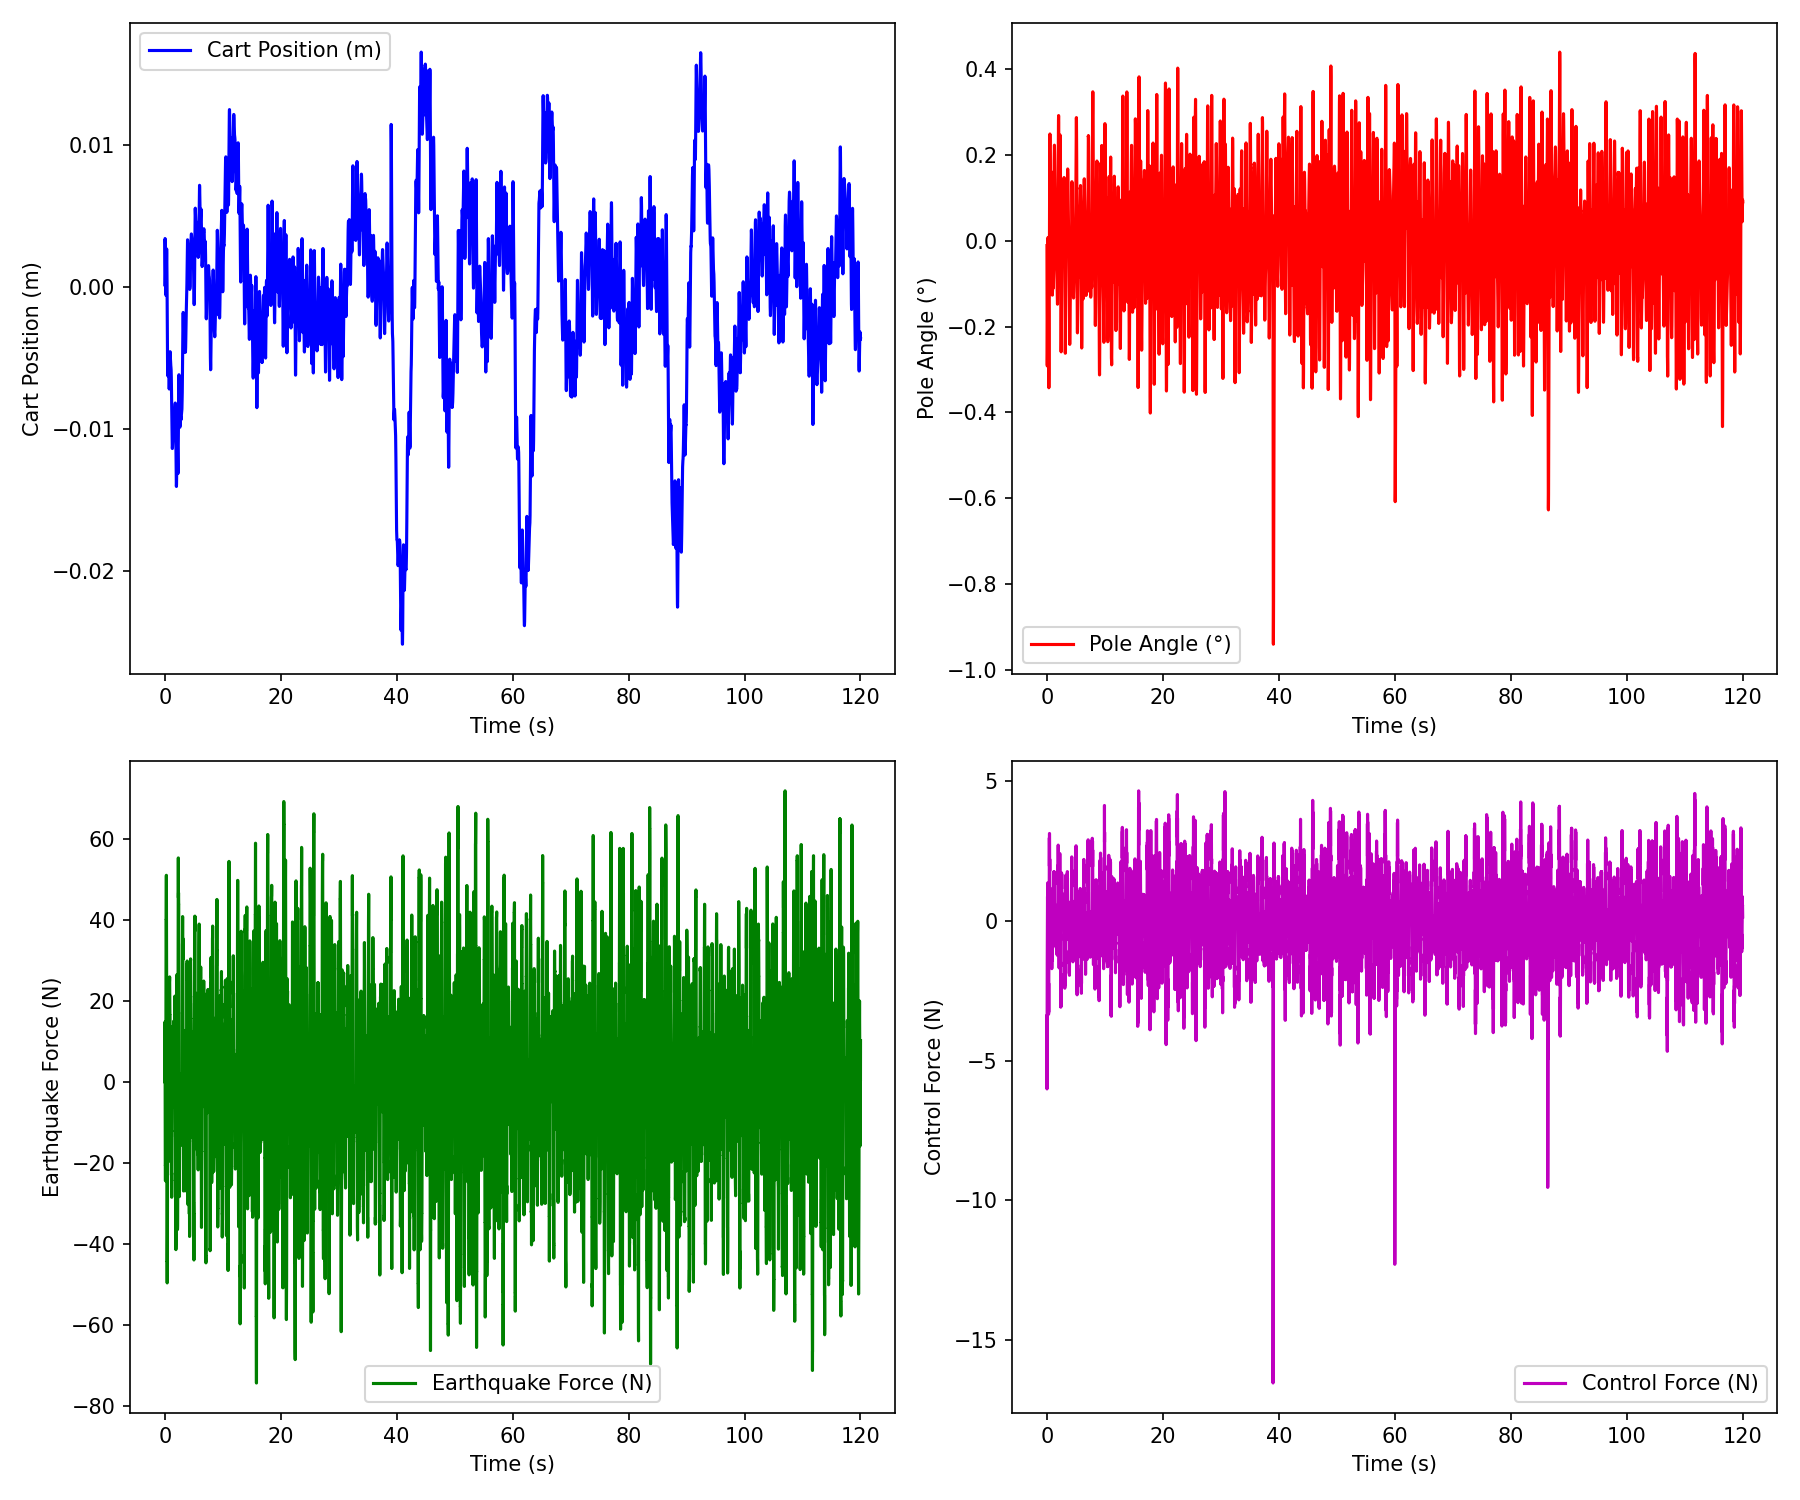
\includegraphics[width=0.9\linewidth]{cart_pole_lqr_results.png}
    \caption{Representative response of the final tuned LQR controller. Replace this figure with the actual output plot from the simulation.}
    \label{fig:lqr_results}
\end{figure}

\section{Deep Q-Network (DQN) Extension}

As an extra-credit extension, a Deep Q-Network (DQN) controller was implemented to provide a model-free reinforcement learning baseline for the cart-pole problem. Whereas the LQR controller used a linearized analytical model and full-state feedback, the DQN controller learned a policy from interaction data using reward-driven training.

\subsection{Controller Formulation}

The DQN used the same state vector as the LQR controller,
\[
x_s =
\begin{bmatrix}
x & \dot{x} & \theta & \dot{\theta}
\end{bmatrix}^T,
\]
but replaced the continuous LQR control law with a discrete action policy. The controller selected from a finite set of candidate force values of the form
\[
u \in \{-15,\,-10,\,-5,\,-2,\,0,\,2,\,5,\,10,\,15\}\,\text{N}.
\]
A neural network was trained to estimate the action-value function \(Q(x_s,u)\), and the control action was selected as the force associated with the largest predicted Q-value.

\subsection{Training Procedure}

Training was performed in a simplified Python cart-pole environment using the same state definition and similar physical parameters as the assignment system. The reward function was shaped to encourage upright pole stabilization, low cart displacement, reduced velocity and angular velocity, and modest control effort. A replay buffer, target network, and \(\epsilon\)-greedy exploration strategy were used during training.

The trained DQN model was then evaluated in the provided ROS2/Gazebo simulation environment using the same cart-pole visualization and earthquake disturbance framework used for the LQR controller.

\subsection{Performance Observations}

The DQN controller was able to learn meaningful stabilizing behavior during training and demonstrated improvement in episode reward over time. However, in the final simulation environment, the DQN controller did not outperform the hand-tuned LQR controller. The LQR controller remained more stable, more consistent, and better behaved under disturbance.

Several factors likely contributed to this result. First, the LQR controller directly exploited a model-based linearized representation of the system, whereas the DQN relied on data-driven policy learning. Second, the DQN used a discrete action set, which limited force resolution relative to the continuous-valued LQR command. Third, the DQN was trained in a simplified environment and then transferred into the full simulation, introducing a mismatch between training and evaluation dynamics.

\subsection{Interpretation}

Although the DQN controller did not exceed the performance of the final tuned LQR controller, the reinforcement learning extension was still useful as a comparison study. It demonstrated that a model-free controller can learn partial stabilization behavior for the cart-pole problem, but that a well-tuned model-based controller remains highly competitive for this structured regulation task.

\subsection{Figures}
\begin{figure}[H]
    \centering
    
\includegraphics[width=0.9\linewidth]{cart_pole_dqn_results.png}
    \caption{Representative response of the trained DQN controller. Replace this figure with the actual output plot from the DQN simulation.}
    \label{fig:dqn_results}
\end{figure}
\begin{figure}[H]
    \centering
    
\includegraphics[width=0.85\linewidth]{dqn_training_rewards.png}
    \caption{DQN training reward as a function of episode number.}
    \label{fig:dqn_training_rewards}
\end{figure}
\begin{figure}[H]
    \centering
    
\includegraphics[width=0.85\linewidth]{dqn_training_loss.png}
    \caption{DQN training loss during optimization.}
    \label{fig:dqn_training_loss}
\end{figure}

\begin{table}[H]
\centering
\caption{Comparison between final tuned LQR controller and DQN controller.}
\label{tab:lqr_dqn_compare}
\begin{tabular}{lcc}
\toprule
Metric & LQR & DQN \\
\midrule
Stable operation duration (s) & [fill] & [fill] \\
Maximum cart displacement (m) & [fill] & [fill] \\
Maximum pole angle deviation (deg) & [fill] & [fill] \\
Average control effort (N) & [fill] & [fill] \\
Qualitative robustness & High & Moderate / Lower \\
\bottomrule
\end{tabular}
\end{table}

\section{Discussion}
The final controller exhibited several important behaviors.

First, it was significantly more robust to hard initial conditions than earlier tuning attempts. In particular, reducing $x_{\max}$ improved the controller's ability to keep the cart centered and reduced large-amplitude oscillations about the origin. This indicates that stronger penalty on cart displacement was beneficial in preventing excessive rail excursions during recovery.

Second, the final value of $\dot{\theta}_{\max}=0.9$ provided a better damping tradeoff than nearby values. Larger values weakened damping and caused visible oscillation growth, while smaller values tended to produce a more overreactive response.

Third, reducing $u_{\max}$ to 15 improved consistency across trials. Although the controller could appear slightly twitchy during the initial transient, the oscillation gradually decayed and the control effort naturally reduced as the cart returned toward the center. This was preferable to a more aggressive controller that performed exceptionally well only in favorable cases but less consistently overall.

Finally, increasing $\theta_{\max}$ from \SI{5}{\degree} to \SI{6}{\degree} reduced the transient recovery time. This suggests that the previous angular penalty was slightly too strict, and relaxing it slightly improved practical performance.

Overall, the final controller should be interpreted as a robustly tuned local stabilizer rather than a globally optimal controller for all possible initial conditions. Since the cart-pole is regulated using a linear controller around the upright equilibrium, some very large deviations are naturally harder to recover from than mild disturbances.

An additional DQN-based reinforcement learning controller was also implemented as an extra-credit extension. While the DQN learned stabilizing behavior and improved substantially during training, it did not match the final hand-tuned LQR controller in the full simulation environment. This result is reasonable, since the LQR controller directly leveraged an analytical model of the system and produced continuous-valued control, whereas the DQN relied on discretized actions and was trained in a simplified environment before transfer to Gazebo.

\section{Conclusion}
An LQR controller was successfully tuned for the cart-pole earthquake disturbance problem using Bryson's Rule as a principled starting point and manual refinement to improve robustness and transient response. The final tuned controller parameters were
\[
x_{\max}=1.2,\quad
\dot{x}_{\max}=3,\quad
\theta_{\max}=\SI{6}{\degree},\quad
\dot{\theta}_{\max}=0.9,\quad
u_{\max}=15.
\]

Compared to the initial Bryson controller, the final tuning improved consistency, reduced oscillation magnitude, improved centering, and maintained low control effort after the transient period. The results demonstrate that Bryson's Rule is an effective initialization method, but manual tuning is still necessary to obtain strong practical performance under disturbance.

In addition to the required LQR tuning study, a DQN-based reinforcement learning controller was implemented as an extra-credit extension. The DQN successfully learned nontrivial stabilizing behavior, but in final simulation testing it did not surpass the performance of the hand-tuned LQR controller. This comparison highlights an important result: for a structured regulation problem with a reliable linearized model, a carefully tuned model-based controller can outperform a basic model-free reinforcement learning approach in both consistency and disturbance rejection.

\end{document}